\selectlanguage{english}
\chapter{Object reconstruction in CMS}
\label{Chapter1}
\newcommand{\cPqb}{\ensuremath{\cmsSymbolFace{b}}}
%SourceDoc tesi.tex

Event reconstruction in CMS is based on the Particle-Flow algorithm \cite{ParticleFlow} aims to reconstruct and identify each individual particle in an event, with an optimized combination of all subdetector information, \figurename~\ref{ParticleFlow}. In this process, the identification of the particle type (photon, electron, muon, charged hadron, neutral hadron) plays an important role in the determination of the particle direction and energy. Photons (\eg  coming from \Pgpz decays or from electron bremsstrahlung) are identified as ECAL energy clusters not linked to the extrapolation of any charged particle trajectory to the ECAL. Electrons %(\eg  coming from photon conversions in the tracker material or from \cPqb-hadron semileptonic decays)%
are identified as a primary charged particle track and potentially many ECAL energy clusters corresponding to this track extrapolated to the ECAL and to possible bremsstrahlung photons emitted along the way through the tracker material. Muons %(\eg  from \cPqb-hadron semileptonic decays)%
are identified as a track in the central tracker consistent with either a track or several hits in the muon system, associated with an energy deficit in the calorimeters. Charged hadrons are identified as charged particle tracks neither identified as electrons, nor as muons. Finally, neutral hadrons are identified as HCAL energy clusters not linked to any charged hadron trajectory, or as ECAL and HCAL energy excesses with respect to the expected charged hadron energy deposit.
%The energy of photons is directly obtained from the ECAL measurement, corrected for zero-suppression effects. The energy of electrons is determined from a combination of the track momentum at the main interaction vertex, the corresponding ECAL cluster energy, and the energy sum of all bremsstrahlung photons attached to the track. The energy of muons is obtained from the corresponding track momentum. The energy of charged hadrons is determined from a combination of the track momentum and the corresponding ECAL and HCAL energy, corrected for zero-suppression effects and for the response function of the calorimeters to hadronic showers. Finally, the energy of neutral hadrons is obtained from the corresponding corrected ECAL and HCAL energy.
%For each event, hadronic jets are clustered from these reconstructed particles using the infrared and collinear safe anti-$k_{t}$ algorithm~\cite{Cacciari:2008gp, Cacciari:2011ma} with a distance parameter of 0.4. The jet momentum is determined as the vectorial sum of all particle momenta in the jet, and is found from simulation to be within 5 to 10\% of the true momentum over the whole $p_{t}$ spectrum and detector acceptance. Additional proton-proton interactions within the same or nearby bunch crossings can contribute additional tracks and calorimetric energy depositions to the jet momentum. To mitigate this effect, tracks identified to be originating from pileup vertices are discarded and an offset correction is applied to correct for remaining contributions. Jet energy corrections are derived from simulation to bring measured response of jets to that of particle level jets on an average. In situ measurements of the momentum balance in dijet, $\text{photon} + \text{jet}$, $\PZ + \text{jet}$, and multijet events are used to account for any residual differences in jet energy scale in data and simulation~\cite{Khachatryan:2016kdb}. The jet energy resolution amounts typically to 15\% at 10 GeV, 8\% at 100 GeV, and 4\% at 1 TeV. Additional selection criteria are applied to each jet to remove jets potentially dominated by anomalous contributions from various subdetector components or reconstruction failures.
\begin{figure}[htbp]
\centering
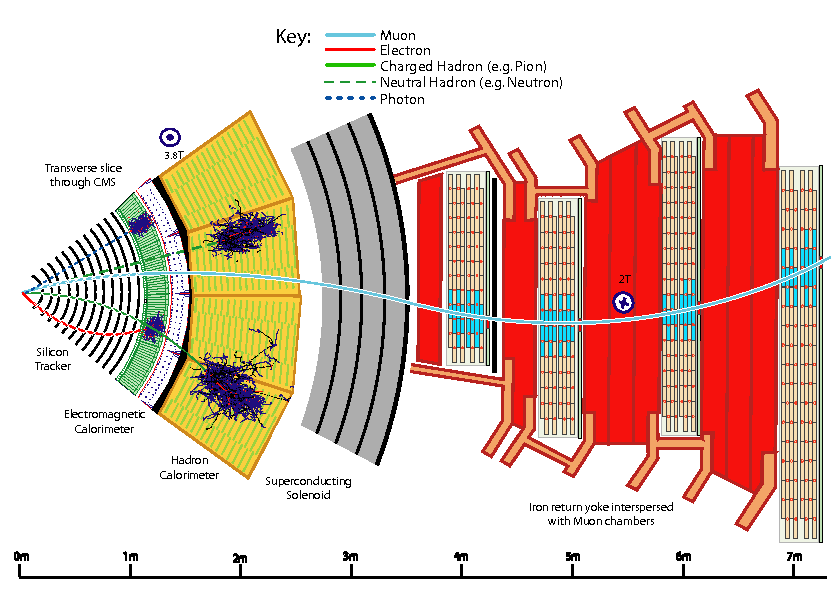
\includegraphics[width=0.7\textwidth]{Images/ParticleFlow}
\caption{Particle interaction and reconstruction in a transverse slice of the CMS detector, from the beam pipe to the muon detector.}
\label{ParticleFlow}
\end{figure}

\section{Track reconstruction}
Track reconstruction aims to obtain estimates for the momentum and position parameters of the charged particles from the hits collected by the tracker detector \cite{Track}. The tracking software at CMS is commonly referred to as the Combinatorial Track Finder (CTF), which is an adaptation of the combinatorial Kalman filter (KF \cite{KF_1, KF_2}), which in turn is an extension of the Kalman filter \cite{KF_1}. The collection of reconstructed tracks is produced by multiple passes (iterations) of the CTF track reconstruction sequence, in a process called iterative tracking. The basic idea of iterative tracking is that the initial iterations search for tracks that are easiest to find (e.g., of relatively large \pt\, and produced near the interaction region). After each iteration, hits associated with tracks are removed, thereby reducing the combinatorial complexity, and simplifying subsequent iterations in a search for more difficult classes of tracks (e.g., low \pt, or greatly displaced tracks). Each iteration proceeds in four steps: seed generation, track finding, track fitting and track selection.
\subsection{Seed generation}
The seeds define the starting trajectory parameters and associated uncertainties of potential tracks. In the quasi-uniform magnetic field of the tracker, charged particles follow helical paths and therefore five parameters are needed to define a trajectory. The seed generation algorithm is controlled by two main sets of parameters: seeding layers and tracking regions. The seeding layers are pairs or triplets of detector layers in which hits are searched for. The tracking regions specify the limits on the acceptable track parameters, including the minimum pT, and the maximum transverse and longitudinal distances of closest approach to the assumed production point of the particle, taken to be located either at the centre of the reconstructed beam spot or at a pixel vertex. If the seeding layers correspond to pairs of detector layers, then seeds are constructed using one hit in each layer. A hit pair is accepted as a seed if the corresponding track parameters are consistent with the requirements of the tracking region. If the seeding layers correspond to triplets of detector layers, then, after pairs of hits are found in the two inner layers of each triplet, a search is performed in the outer detector layer for another hit. If the track parameters, derived from the three hits, are compatible with the tracking region requirements, the seed is accepted.
\subsection{Track finding}
The track-finding module of the CTF algorithm is based on the Kalman filter method. The filter begins with a coarse estimate of the track parameters provided by the trajectory seed, and then builds track candidates by adding hits from successive detector layers, updating the parameters at each layer. The information needed at each layer includes the location and uncertainty of the detected hits, as well as the amount of material crossed, which is used to estimate the effects of multiple Coulomb scattering and energy loss. The track finding is implemented in four different steps. All resulting track candidates found at each layer are then propagated to the next compatible layers, and the procedure is repeated until a termination condition is satisfied. However, to avoid a rapid increase in the number of candidates, only a limited number (default is 5) of the candidates are retained at each step, with the best candidates chosen based on the normalized $\chi^2$. Once the search for hits in the outward direction reveals a minimum number of valid hits, an inwards search is initiated for additional hits.
\subsection{Track fitting}
For each trajectory, the track-finding stage yields a collection of hits and an estimate of the track parameters. However, the full information about the trajectory is only available at the final hit of the trajectory (when all hits are known). Furthermore, the estimate can be biased by constraints, such as a beam spot constraint applied to the trajectory during the seeding stage. The trajectory is therefore refitted using a Kalman filter and smoother. The Kalman filter is initialized at the location of the innermost hit, with the trajectory estimate obtained by performing a Kalman filter fit to the innermost hits (typically four) on the track. The fit then proceeds in an iterative way through the full list of hits, from the inside outwards, updating the track trajectory estimate sequentially with each hit. For each valid hit, the estimated hit position uncertainty is reevaluated using the current values of the track parameters.
\subsection{Track selection}
In order to reduce fake tracks (reconstructed track not associated with a charged particle), tracks are selected on the basis of the number of layers that have hits, whether their fit yielded a good $\chi^2$/dof, and how compatible they are with originating from a primary interaction vertex. The fraction of fake tracks decreases roughly exponentially as a function of the number of layers in which the track has associated hit: weaker selection criteria can be applied for tracks having many hit layers but these criteria become more stringent for tracks with relatively few hit layers. Different kind of criteria can be chosen according to the requirements: from loose to high-purity reducing the efficiency and fake rate. After the track selection is complete, the tracks found by each of the six iterations are merged into a single collection.

\section{Vertices}
The goal of primary-vertex reconstruction [50] is to measure the location, and the associated un-certainty, of all proton-proton interaction vertices in each event, including the signal vertex and any vertices from pileup collisions, using the available reconstructed tracks. It consists of three steps:
\begin{itemize}
\item selection: imposing several requirements, tracks consistent with being produced promptly in the primary interaction region are selected
\item clustering: the selected tracks are clustered on the basis of their z-coordinates at their point of closest approach to the centre of the beam spot. In this step, all proton-proton interactions in the same LHC bunch crossing are reconstructed. The clustering is performed using a deterministic annealing (DA) algorithm \cite{DA_vertex}
\item fitting: all the vertices containing at least two tracks are then fitted using an adaptive vertex fitter \cite{AVF_vertex} to compute the best estimate of vertex parameters, including 3-D poistion and coordinate covariance matrix, as well as the indicators for the success of the fit, such as the number of degrees of freedom for the vertex, and weights of the tracks used in the vertex.
\end{itemize}

\section{Photons}
Photons \cite{photons}, for use as signals or signatures in measurements and searches, rather than for use in the construction of jets or missing transverse energy, are reconstructed from energy deposits in the ECAL using algorithms that constrain the clusters to the size and shape expected for electrons and photons with \pt  $\ge$15 GeV. The reconstructed ECAL showers are generally limited to a fiducial region excluding the last two crystals at each end of the barrel ($|\eta | <$ 1.4442). The outer circumferences of the endcaps are obscured by services passing between the barrel and the endcaps, and this area is removed from the fiducial region by excluding the first ring of trigger towers of the endcaps ($|\eta | >$ 1.566). The fiducial region terminates at $|\eta|$ = 2.5 where the tracker coverage ends.The photon reconstruction proceeds through several steps: 
\begin{itemize}
\item calibration: the calorimeter signals in data must be calibrated and corrected for several detector effects
\item clusterisation: clustering algorithms collect the energy from radiating electrons and converted photons that gets spread in the $\phi$ direction by the magnetic field; these algorithms are evolved from fixed matrices of 5 x 5 crystals, which provide the best reconstruction of unconverted photons, by allowing extension of the energy collection in the $\phi$ direction, to form "superclusters"
\item correction of cluster energy: main effects (\eg variation of longitudinal containment, variation of lateral containment or variation in the amount of energy absorbed before reaching the ECAL for showers starting before the ECAL) force to correct the initial sum of energy deposits
\end{itemize}

\section{Electrons}
Electrons \cite{electrons} are reconstructed by associating a track reconstructed in the silicon detector with a cluster of energy in the ECAL. A mixture of a stand-alone approach \cite{electrons_2} and the complementary global particle-flow algorithm is used to maximize the performance. The electron energy usually spreads out over several crystals of the ECAL. This spread can be quite small when electrons lose little energy via bremsstrahlung before reaching ECAL. To measure the initial energy of the electron accurately, it is essential to collect the energy of the radiated photons that mainly spreads along the $\phi$ direction because of the bending of the electron trajectory in the magnetic field. The spread in the $\eta$ direction is usually negligible, except for very low \pt~(\pt $<$ 5GeV). Two clustering algorithms, the hybrid algorithm in the barrel, and the "multi-5x5" in the endcaps, are used for this purpose. \\
The starting point of the hybrid algorithm is a seed crystal, defined as the one containing most of the energy deposited in any considered region: arrays of 5 x 1 crystals in $\eta$ x $\phi$ are added around the seed crystal, in a range of $N_{steps}$ crystals in both directions of $\phi$ if their energies exceed a minimum threshold. The contiguous arrays are grouped into clusters, with each distinct cluster required to have a seed array with energy greater than a threshold in order to be collected in the final global cluster, called the supercluster seed-array (SC). \\
The multi-5x5 algorithm is used in the ECAL endcaps (EE), where crystals are not arranged in an $\eta \times \phi$ geometry. It starts with the seed crystals, the ones with local maximal energy relative to their four direct neighbours. Around these seeds and beginning with the largest $E_T$, the energy is collected in clusters of 5x5 crystals, that can partly overlap. These clusters are then grouped into an SC if their total $E_T$ is greater then a minimum, within a range in $\eta$ of $\pm \eta_{range}$, and a $\phi$ of $\pm \phi_{range}$ around each seed crystal. The SC energy corresponds to the sum of the energies of all its clusters. The SC position is calculated as the energy-weighted mean of the cluster positions. \\
In addition, as part of the PF-reconstruction algorithm, another clustering algorithm is introduced that aims at reconstructing the particle showers individually. The PF clusters are reconstructed by aggregating around a seed all contiguous crystals with energies of two standard deviations above the electronic noise observed at the beginning of the data-taking run \\
Electron tracks can be reconstructed in the full tracker using the standard KF track reconstruction procedure used for all charged particles. However, the large radiative losses for electrons in the tracker material compromise this procedure and lead in general to a reduced hit-collection efficiency (hits are lost when the change in curvature is large because of bremsstrahlung), as well as to a poor estimation of track parameters. For these reasons, a dedicated tracking procedure is used for electrons.
\subsection{Seeding}
Consists of finding and selecting the two or three first hits in the tracker from which the track can be initiated. The seeding is of primary importance since its performance greatly affects the reconstruction efficiency. Two complementary algorithms are used and their results combined. The ECAL-based seeding starts from the SC energy and position, used to estimate the electron trajectory in the first layers of the tracker, and selects electron seeds from all the reconstructed seeds. The tracker-based seeding relies on tracks that are reconstructed using the general algorithm for charged particles, extrapolated towards the ECAL and matched to a SC. 
\subsection{Tracking}
The selected electron seeds are used to initiate electron-track building, which is followed by track fitting. The track building is based on the combinatorial KF method, which for each electron seed proceeds iteratively from the track parameters provided in each layer, including one-by-one the information from each successive layer. The electron energy loss is modelled through a Bethe-Heitler function. To follow the electron trajectory in case of bremsstrahlung and to maintain good efficiency, the compatibility between the predicted and the found hits in each layer is chosen not to be too restrictive. When several hits are found compatible with those predicted in a layer, then several trajectory candidates are created and developed, with a limit of five candidate trajectories for each layer of the tracker. At most, one missing hit is allowed for an accepted trajectory candidate, and, to avoid including hits from converted bremsstrahlung photons in the reconstruction of primary electron tracks, an increased $\chi^2$ penalty is applied to trajectory candidates with one missing hit. Once the hits are collected, a Gaussian sum filter (GSF \cite{GSF}) fit is performed to estimate the track parameters. The energy loss in each layer is approximated by a mixture of Gaussian distributions. A weight is attributed to each Gaussian distribution that describes the associated probability. 
\subsection{Electron particle-flow clustering}
The PF clustering of electrons is driven by GSF tracks, and is independent of the way they are seeded. For each GSF track, several PF clusters, corresponding to the electron at the ECAL surface and the bremsstrahlung photons emitted along its trajectory, are grouped together. The PF cluster corresponding to the electron at the ECAL surface is the one matched to the track at the exit of the tracker. Since most of the material is concentrated in the layers of the tracker, for each layer a straight line is extrapolated to the ECAL, tangent to the electron track, and each matching PF cluster is added to the electron PF cluster. Most of the bremsstrahlung photons are recovered in this way, but some converted photons can be missed. For these photons, a specific procedure selects displaced KF tracks through a dedicated MVA algorithm, and kinematically associates them with the PF clusters. In addition, for ECAL-seeded isolated electrons, any PF clusters matched geometrically with the hybrid or multi-5x5 SC are also added to the PF electron cluster.
\subsection{Association between track and cluster}
The electron candidates are constructed from the association of a GSF track and a cluster in the ECAL. For ECAL-seeded electrons, the ECAL cluster associated with the track is simply the one reconstructed through the hybrid or the multi-5x5 algorithm that led to the seed. For electrons seeded only through the tracker-based approach, the association is made with the electron PF cluster.

\section{Muons}
\subsection{Reconstruction}
\label{sec:MuonReconstruction}
Muons are first reconstructed independently in the inner tracker (tracker track) and in the muon system (standalone-muon track) \cite{muons, muons_2}. Tracker tracks are built using an iterative approach, running a sequence of tracking algorithms each with slightly different logic. After each iteration step, hits that have been associated with reconstructed tracks are removed from the set of input hits to be used in the following step. Standalone-muon tracks are built instead by exploiting information from muon subdetectors to gather all CSC, DT, and RPC information along a muon trajectory using a Kalman-filter technique (KF, \cite{KF_muon}). Reconstruction starts from seeds made up of groups of DT or CSC segments. \\
Based on tracker track and Standalone-muon, two reconstruction approaches are used:
\begin{itemize}
\item Global Muon reconstruction (outside-in): for each standalone-muon track, a matching tracker track is found by comparing parameters of the two tracks propagated onto a common surface. A global-muon track is fitted combining hits from the tracker track and standalone-muon track, using the KF technique . At large transverse momenta, \pt  $\ge$ 200 GeV, the global-muon fit can improve the momentum resolution compared to the tracker-only fit
\item Tracker Muon reconstruction (inside-out): in this approach, all tracker tracks with \pt $>$ 0.5 GeV and total momentum p $>$ 2.5 GeV are considered as possible muon candidates and are extrapolated to the muon system taking into account the magnetic field, the average expected energy losses, and multiple Coulomb scattering in the detector material. If at least one muon segment (i.e., a short track stub made of DT or CSC hits) matches the extrapolated track, the corresponding tracker track qualifies as a Tracker Muon. Track-to-segment matching is performed in a local (chamber) coordinate system, where local x is the best-measured coordinate (in the r-$\phi$ plane) and local y is the coordinate orthogonal to it. The extrapolated track and the segment are considered to be matched if the distance between them in local x is less than 3 cm or if the value of the pull for local x is less than 4, where the pull is defined as the difference between the position of the matched segment and the position of the extrapolated track, divided by their combined uncertainties.
\end{itemize}
Tracker Muon reconstruction is more efficient than the Global Muon reconstruction at low momenta, p $\ge$ 5GeV, because it requires only a single muon segment in the muon system, whereas Global Muon reconstruction is designed to have high efficiency for muons penetrating through more than one muon station and typically requires segments in at least two muon stations. 
Reconstructed muons are fed into the CMS PF algorithm that applies a set of selection criteria to candidates reconstructed with the standalone, global, or tracker muon algorithms. The requirements are based on various quality parameters from the muon reconstruction as well as make use of information from other CMS subdetectors. 
\subsubsection{High-pT muon}
CMS has also developed specialised algorithms for high-pT muon (TeV-muon) reconstruction and momentum assignment. As the muon passes through the steel of the magnet return yoke, multiple scattering and radiative processes can alter the muon trajectory. In particular, this radiative processes can result in large energy losses and can produce electromagnetic showers giving rise to additional hits in the muon chambers. As a consequence, the estimate of the muon momentum at the production vertex can be significantly different from its true value. Therefore, for each muon a set of specially developed TeV-muon track fits is performed:
\begin{itemize}
\item Tracker plus first muon station (TPFMS): this algorithm refits the global-muon track using hits from the tracker and the innermost muon station for reduced sensitivity to possible showering deeper in the muon system due to the larger amount of iron traversed by the muon.
\item Picky: this algorithm again starts with the hit list of the global-muon track, but, in chambers appearing to have hits from showers (determined by the hit occupancy of the chamber), retains only the hits that, based on a $\chi^2$ comparison, are compatible with the extrapolated trajectory.
\item Dynamic truncation (DYT): this fit takes into account possible energy losses from radiative processes and tries to avoid hits produced after a large energy loss in the muon system. For every silicon tracker track identified as belonging to a muon by the global fit, the result of the tracker-only fit is propagated out to the muon stations and attempts are made to add compatible muon hits to the fit. For each hit the compatibility between the extrapolated tracker track and the reconstructed segment in the muon chambers is calculated, using an estimator that in absence of correlation reduces to a $\chi^2$.
\end{itemize}
To further improve the resolution at high \pt, mainly by reducing the tails of the momentum resolution distribution, combinations of the above algorithms can be used. Momentum assignment is so performed by the \textit{Tune P} algorithm, which chooses the best muon reconstruction between global-track, tracker-track, TPFMS, Picky, and DYT. The selection is made on a track-by-track basis, using the track fit $\chi^2$/ndf tail probability and the relative \pt\ measurement error $\sigma_{p_T}$/\pt.
\subsection{Identification}
\label{sec:Identification}
\label{ID}
According to the required identification efficiency and purity, different selection based on a set of variables can be applied. Some variables are based on muon reconstruction,  such as track fit $\chi^2$, the number of hits per track (either in the inner tracker or in the muon system, or both), or the degree of matching between tracker tracks and standalone-muon tracks (for global muons). Other variables exploit inputs from outside the reconstructed muon track, such as compatibility with the primary vertex (the reconstructed vertex with the largest value of summed
physics-object $p_T^{2}$). Using these variables, the main identification types of muons used in CMS physics analyses include:
\begin{itemize}
\item Loose muon Identification (Loose ID): aims to identify prompt muons originating at the primary vertex, and muons from light and heavy flavor decays, as well as maintain a low rate of the misidentification of charged hadrons as muons.  A loose muon is a muon selected by the PF algorithm that is also either a tracker or a global muon.
\item Medium muon ID: optimised for prompt muons and for muons from heavy flavor decay.  A medium muon is a loose muon with a tracker track that uses hits from more than 80\% of the inner tracker layers it traverses.  According if the muon is only reconstructed as a tracker muon or as both a tracker muon and a global muon, the
muon segment compatibility need to be greater than a fixed threshold. The  constraints  on  the  segment  compatibility  were  tuned  after  application  of  the other constraints to target an overall efficiency of 99.5\% for muons from simulated W and Z events.
\item Tight muon ID: aims  to  suppress  muons  from  decay  in  flight  and  from  hadronic punch-through.  A tight muon is a loose muon with a tracker track that uses hits from at least six layers of the inner tracker including at least one pixel hit. The muon must be reconstructed as both a tracker muon and a global muon. The tracker muon must have segment matching in at least two of the muon stations. The global muon fit must have $\chi^2$/dof $<$10 and include at least one hit from the muon system.  A tight muon must be compatible with the primary vertex, having a transverse impact parameter $|dxy| <$ 0.2 cm and a longitudinal impact parameter $|dz| <$0.5 cm. This selection is used in many physics analyses in CMS, in particular in the measurements of inclusive W and Z cross sections.
\item Soft muon ID: optimized for low-\pt\ muons for B-physics and quarkonia analyses. A soft muon is a tracker muon with a tracker track that satisfies a high purity flag and uses hits from at least six layers of the inner tracker including at least one pixel hit. The tracker muon reconstruction must have tight segment matching,  having pulls less than 3 both in local x and in local y.  A soft muon is loosely compatible with the primary vertex, having $|dxy| <$ 0.3 cm and $|dz| <$20 cm.
\item High-pT ID: optimized for muons with \pt $>$200 GeV.  A high momentum muon is reconstructed as both a tracker muon and a global muon. The requirements on the tracker track, the tracker muon, and the transverse and longitudinal impact parameters are the same as for a tight muon, as well as the requirement that there be at least one hit from the muon system for the global muon. However, in contrast to the tight muon, the requirement on the global muon fit $\chi^2$/dof is removed.  The removal of the $\chi^2$/dof requirement prevents inefficiencies at high \pt when muons radiate large electromagnetic showers as they pass through the steel flux-return yoke, giving rise to additional hits in the muon chambers. A requirement on the relative \pt uncertainty, $\sigma_{p_T}/p_T <0.3$ is used to ensure a proper momentum measurement.
\end{itemize}
\subsection{Isolation}
To distinguish between prompt muons and those from weak decays within jets, the isolation of a muon is evaluated  relative  to  its \pt by  summing  up  the  energy  of all particles in  geometrical  cones with $\Delta R = \sqrt{\Delta\eta^2+\Delta\phi^2}$, surrounding the muon. One strategy sums reconstructed tracks (track based isolation), while another uses charged hadrons and neutral particles coming from PF (PF isolation). For the computation of PF isolation [17], the \pt of charged hadrons within the $\Delta R$ cone originating from the primary vertex are summed together with the energy sum of all neutral particles (hadrons and photons) in the cone.   The contribution from pileup to the neutral particles is corrected by computing the sum of charged hadron deposits originating from pileup vertices, scaling it by a factor of 0.5,  and subtracting this from the neutral hadron and photon sums to give the corrected energy sum from neutral particles.  The factor of 0.5 is estimated from simulations to be approximately the ratio of neutral particle to charged hadron production in inelastic proton-proton collisions.  The corrected energy sum from neutral particles is limited to be positive or zero. For both strategies, tight and loose working points are defined to achieve efficiencies of 95\% and 98\%, respectively.  They are tuned using simulated tight muons from $Z\to\mu^+\mu^-$ decays with \pt $>$ 20 GeV.  The values for the tight and loose working points for PF isolation within $\Delta R<$ 0.4 are 0.15 and 0.25, respectively, while the values for track based isolation within $\Delta R <$ 0.3 are 0.05 and 0.10.  The efficiency of the working points to reject muons in jets was tested in simulated multi-jet QCD events (events comprised uniquely of jets produced through the strong interaction) and simulated events containing a W boson plus one or more jets (W+jets).

\section{Taus}
Due to its short life time ($c\tau = 87 \mu m$), $\tau$ lepton decays before reaching the detector elements. In two thirds of the cases, $\tau$ leptons decay hadronically, typically into one or three charged mesons (predominantly $\pi^\pm$), often accompanied by neutral pions (decaying via $\pi^0 \to \gamma\gamma$), and a $\nu_\tau$. In the last third ($\approx 35\%$), $\tau$ decays into lighter leptons. Algorithms that use final-state photons and charged hadrons to identify hadronic decays of $\tau$ leptons ($\tau_h$) through the reconstruction of the intermediate resonances have been developed: the hadron plus strips (HPS) and the tau neural classifier (TaNC) with this last one used to cross check the first. \\
Both algorithms start the reconstruction of a $\tau_h$ candidate from a PF jet, whose four-momentum is reconstructed using the anti-$k_T$~\cite{Jet_Cacciari:2008gp, Jet_Cacciari:2011ma} algorithm with a distance parameter R = 0.5. Using a PF jet as an initial seed, the algorithms first reconstruct the $\pi^0$ components of the $\tau_h$, then combine them with charged hadrons to reconstruct the tau decay mode and calculate the tau four-momentum and isolation quantities.
\subsection{HPS algorithm}
HPS algorithm in based on the reconstruction in "strips" of photons produced by the $\pi^0$ decays and electrons produced by the photon conversions in the tracker material. The strip reconstruction starts by centering a strip on the most energetic electromagnetic particle within the PF jet. The algorithm then searches for other electromagnetic particles within a window of size $\Delta\eta$ = 0.05 and $\Delta\phi$ = 0.20 centered on the strip center. If other electromagnetic particles are found within that window, the most energetic one gets associated with the strip and the strip four-momentum is recalculated. The procedure is repeated until no further particles are found that can be associated with the strip. Strips satisfying a minimum transverse momentum requirement of $p_T^{strip} >$ 1 GeV are finally combined with the charged hadrons to reconstruct individual $\tau_h$ decay modes.\\
The decay topologies that are considered by the HPS tau identification algorithm are:
\begin{itemize}
\item Single hadron: corresponds to $h^-\nu_\tau$ and $h^-\pi^0\nu_\tau$ decays in which the neutral pions have too little energy to be reconstructed as strips.
\item One hadron + one strip: reconstructs the decay mode $h^-\pi^0\nu_\tau$ in events in which the photons from $\pi^0$ decay are close together on the calorimeter surface.
\item One hadron + two strip: corresponds to the decay mode $h^-\pi^0\nu_\tau$ in events in which photons from $\pi^0$ decays are well separated.
\item Three hadron: corresponds to the decay mode $h^-h^+h^-\nu_\tau$. The three charged hadrons are required to come from the same secondary vertex.
\end{itemize}
The reconstructed tau have also to be isolated which means that no charged hadrons or photons present within an isolation cone of size $\Delta$R = 0.5 around the direction of the $\tau_h$; its momentum have also to match the ($\eta$, $\phi$) direction of the original PF jet within a maximum distance of $\Delta$R = 0.1. 
\subsection{TaNC algorithm}
TaNC algorithm reconstructs the PF $\tau_h$ four-momentum as a sum of the four-momenta of all particles with \pt~above 0.5 GeV in a cone of radius $\Delta$R + 0.15 around the direction of the leading particle. The decay mode is reconstructed from the particles that are contained within the signal cone of the $\tau_h$ candidate by counting the number of tracks and $\pi^0$ meson candidates and is uniquely determined by the multiplicity of reconstructed objects in the signal cone. The signal cone is defined as the region where the $\tau_h$ decay products are expected to be found. 

\section{Jets}
Jets are reconstructed offline from the energy deposits in the calorimeter towers, clustered using the anti-$k_T$ algorithm with a distance parameter of 0.4 (AK4 jets); for studies involving boosted topologies, jets are clustered with a larger distance parameter R = 0.8 (AK8 jets). In this process, the contribution from each calorimeter tower is assigned a momentum, the absolute value and the direction of which are given by the energy measured in the tower, and the coordinates of the tower. The raw jet energy is obtained from the sum of the tower energies, and the raw jet momentum by the vectorial sum of the tower momenta, which results in a nonzero jet mass. The raw jet energies are then corrected to establish a relative uniform response of the calorimeter in $\eta$ and a calibrated absolute response in transverse momentum \pt. Jet momentum is determined as the vectorial sum of all particle momenta in the jet, and is found from simulation to be within 5 to 10\% of the true momentum over the whole \pt\ spectrum and detector acceptance. Additional proton-proton interactions within the same or nearby bunch crossings can contribute additional tracks and calorimetric energy depositions to the jet momentum. To mitigate this effect, tracks identified to be originating from pileup vertices are discarded, and an offset correction is applied to correct for remaining contributions. Jet energy corrections are derived from simulation to bring the measured response of jets to that of particle level jets on average. In situ measurements of the momentum balance in dijet, photon + jet, Z+jet, and multijet events are used to account for any residual differences in jet energy scale in data and simulation. Additional selection criteria are applied to each jet to remove jets potentially dominated by anomalous contributions from various subdetector components or reconstruction failures. The jet energy resolution amounts typically to 15\% at 10 GeV, 8\% at 100 GeV, and 4\% at 1 TeV, to be compared to about 40\%, 12\%, and 5\% obtained when the calorimeters alone are used for jet clustering.
\subsection{Heavy-flavour jets}
Heavy-flavour jets (HF jets) \cite{HF_Jets} are jets originating from bottom or charm quarks: CMS has developed an algorithm to identify these jets from the light ones (the jets coming from lighter quarks). Algorithms for HF jet identification use variables connected to the properties of heavy-flavour hadrons present in jets resulting from the radiation and hadronization of b or c quarks. For instance, the lifetime of hadrons containing b quarks is of the order of 1.5 ps, while the lifetime of c hadrons is 1 ps or less. This leads to typical displacements of a few mm to one cm for b hadrons, depending on their momentum, thus giving rise to displaced tracks from which a secondary vertex (SV) may be reconstructed (\figurename~\ref{bJet_SV}).
\begin{figure}[htbp]
\centering
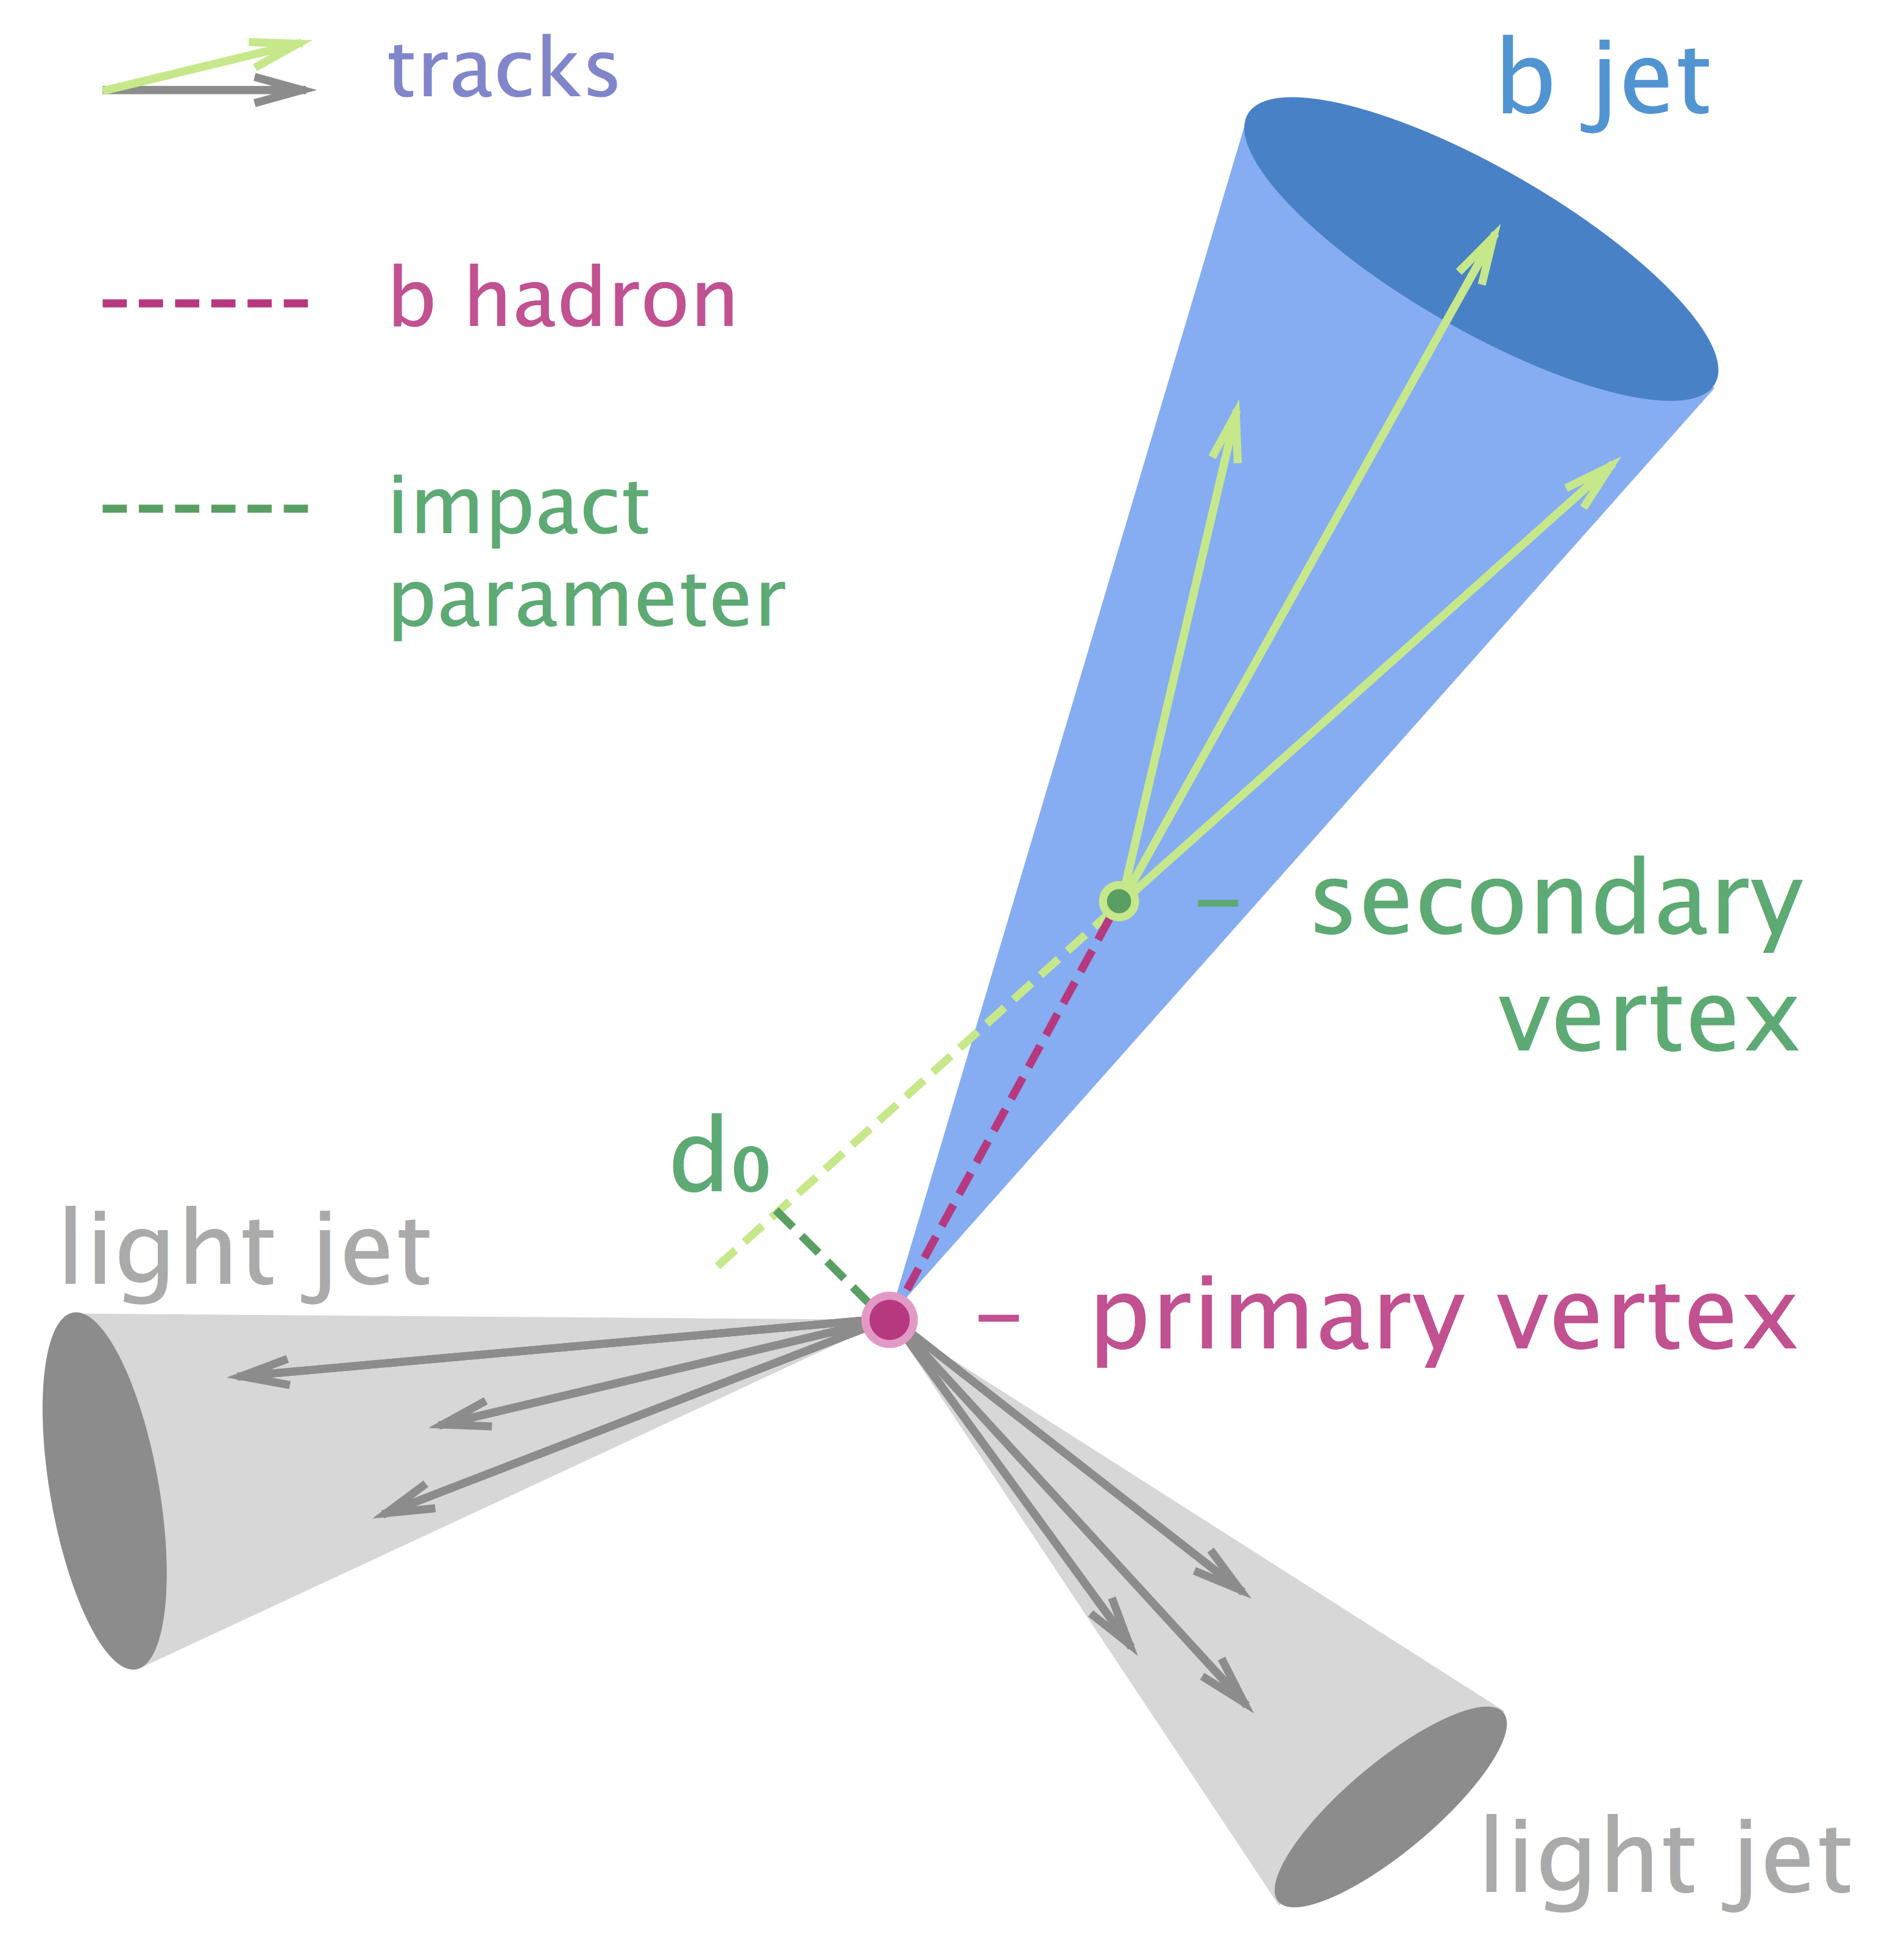
\includegraphics[width=0.35\textwidth]{Images/bJet_SV}
\caption{Illustration of a heavy-flavour jet with a secondary vertex (SV) from the decay of a b or c hadron resulting in charged-particle tracks (including possibly a soft lepton) that are displaced with respect to the primary interaction vertex (PV), and hence with a large impact parameter (IP) value.}
\label{bJet_SV}
\end{figure}
In order to design and optimize heavy-flavour identification techniques, a reliable method is required for assigning a flavour to jets in simulated events. The jet flavour is determined by clustering not only the reconstructed final-state particles into jets, but also the generated b and c hadrons that do not have b and c hadrons as daughters respectively. Jets containing at least one b hadron are defined as b jets; the ones containing at least one c hadron and no b hadron are defined as c jets. The remaining jets are considered to be light-flavour (or "udsg") jets. The properties of the tracks clustered within the jet represent the basic inputs of all heavy-flavour jet identification (tagging) algorithms. Input variables for the tagging algorithms are constructed from the tracks after applying appropriate selection criteria. In particular, the combined multivariate algorithm (cMVA) was developed combining the information from six different b jet identification discriminators with a Boosted Decision Tree.


